
\documentclass[10pt,a4paper,twocolumn]{article}

\usepackage[
    a4paper,
    top=1.65cm,
    bottom=1.65cm,
    left=1.55cm,
    right=1.55cm,
    columnsep=0.55cm
]{geometry}

\usepackage[T1]{fontenc}
\usepackage{lmodern}
\usepackage{microtype}
\usepackage{setspace}
\setlength{\parindent}{1em}
\setlength{\parskip}{2pt}
\linespread{0.97}
\setlength{\columnsep}{0.55cm}
\setlength{\emergencystretch}{2em}

\usepackage{xcolor}
\definecolor{navy}{HTML}{17324D}
\definecolor{teal}{HTML}{168C8C}
\definecolor{muted}{HTML}{526273}
\definecolor{rulecolor}{HTML}{D9E2EC}

\usepackage{titlesec}
\titleformat{\section}
  {\large\bfseries\color{navy}}
  {\thesection.}{0.45em}{}
\titleformat{\subsection}
  {\normalsize\bfseries\color{teal}}
  {\thesubsection}{0.45em}{}

\titlespacing*{\section}{0pt}{8pt}{3pt}
\titlespacing*{\subsection}{0pt}{5pt}{2pt}

\usepackage{booktabs}
\usepackage{tabularx}
\usepackage{array}
\usepackage{tikz}
\usetikzlibrary{arrows.meta, positioning}

\usepackage[hidelinks]{hyperref}
\usepackage{fancyhdr}
\usepackage{balance}

\pagestyle{fancy}
\fancyhf{}
\fancyhead[L]{\small\textcolor{muted}{TASKLY}}
\fancyhead[R]{\small\textcolor{muted}{Student Planner}}
\fancyfoot[C]{\small\textcolor{muted}{\thepage}}
\renewcommand{\headrulewidth}{0.35pt}
\renewcommand{\headrule}{\hbox to\headwidth{\color{rulecolor}\leaders\hrule height \headrulewidth\hfill}}

\setlength{\headheight}{13pt}
\setlength{\textfloatsep}{7pt}
\setlength{\intextsep}{6pt}
\setlength{\abovecaptionskip}{3pt}
\setlength{\belowcaptionskip}{0pt}

\title{
  \vspace{-1.15cm}
  {\Large\bfseries\color{navy}
  Taskly: A Student-Centered Academic Planning Application}\\[5pt]
  {\normalsize\color{teal}
  Design, Implementation, and Software Architecture}
  \vspace{-5pt}
}

\author{
  \normalsize
  Hassan Abdelmajeed \quad
  Yassin Kilani \quad
  Habiba Basel\\[3pt]
  Habiba Khaled \quad
  Mazen Ashraf \quad
  Yasmine Rabie
}

\date{}

\begin{document}
\maketitle
\vspace{-12pt}

\begin{abstract}
University students often manage assignments, courses, deadlines, and
personal commitments across disconnected tools. Taskly is an Android
student-planning application designed to bring academic task management
into a single interface. This paper presents the application's design
objectives, user-facing functionality, and implementation approach,
with emphasis on maintainability, data organization, and usability.
The discussion connects the interface to the underlying application
structure and identifies practical directions for further development.
\end{abstract}

\noindent\textbf{\textcolor{navy}{Keywords---}}
Android, student planner, Jetpack Compose, task management,
mobile application architecture.

\section{Introduction}

Academic planning requires students to track multiple deadlines while
maintaining a clear view of their workload. When tasks and course
information are distributed across separate applications, important
details can become difficult to organize and review.

Taskly addresses this problem by providing a dedicated environment for
academic planning. Its central goal is to make tasks easier to create,
categorize, review, and manage through a consistent Android interface.
Rather than treating task management as an isolated checklist, the
application is structured around the relationship between academic
subjects and their associated work.

The project emphasizes three design priorities: a focused user
experience, clear organization of academic information, and an
implementation structure that can be maintained and extended.

\section{Application Design and Functionality}

Taskly organizes its user experience around the main activities involved
in student planning. Users can work with academic tasks, associate tasks
with subjects, and access task information through purpose-built screens.

\subsection{Task Management}

Task creation and editing are central workflows. A task form provides
a structured place to enter relevant information, while task-list
screens make existing work easier to review. Connecting tasks to
subjects adds academic context and helps users distinguish work across
different courses.

The interface should communicate task state and available actions
consistently. Clear labels, predictable navigation, and reusable
interface elements reduce unnecessary interaction and make common
workflows easier to understand.

\subsection{Interface Design}

The Android interface is implemented with Jetpack Compose, which
supports declarative UI development and reusable composable functions.
This approach allows screens to be assembled from smaller components
and updated in response to application state.

A consistent visual system is important beyond appearance: spacing,
typography, color, and component behavior should reinforce information
hierarchy. Shared components also reduce duplication and make interface
changes easier to apply consistently.

\section{Technical Architecture}

A maintainable mobile application benefits from separating the user
interface from business logic and persistent data. In a layered design,
the UI presents state and forwards user actions, while state-management
components coordinate application behavior and data access.

\begin{figure}[t]
\centering
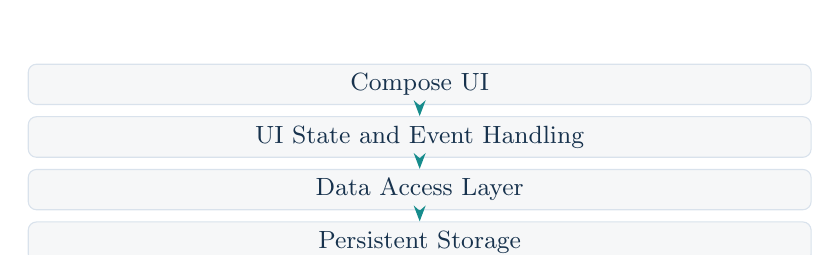
\begin{tikzpicture}[
  node distance=4pt,
  block/.style={
    draw=rulecolor,
    rounded corners=3pt,
    fill=navy!4,
    text=navy,
    align=center,
    minimum width=0.82\columnwidth,
    minimum height=0.48cm,
    font=\small
  },
  arr/.style={-{Stealth[length=2mm]}, thick, color=teal}
]
\node[block] (ui) {Compose UI};
\node[block, below=of ui] (state) {UI State and Event Handling};
\node[block, below=of state] (data) {Data Access Layer};
\node[block, below=of data] (store) {Persistent Storage};

\draw[arr] (ui) -- (state);
\draw[arr] (state) -- (data);
\draw[arr] (data) -- (store);
\end{tikzpicture}
\caption{Conceptual separation of presentation, state management,
data access, and storage.}
\label{fig:architecture}
\end{figure}

Figure~\ref{fig:architecture} illustrates the intended separation of
responsibilities. The presentation layer renders information and
captures user input. The state-management layer coordinates screen
behavior, and the data-access layer isolates storage operations from
the interface. Persistent storage retains application data between
sessions.

This separation improves readability and provides clear boundaries
for testing and future changes. However, the diagram represents a
conceptual architecture; the precise components and data flow should
be aligned with the final implementation.

\subsection{Android Implementation}

Jetpack Compose provides the declarative presentation model. Kotlin
supports concise application logic and type-safe modeling of data.
Together, these technologies allow UI components and application
behavior to be organized into focused units.

The architecture should ensure that composables do not become
responsible for unrelated storage or business rules. Keeping state
ownership explicit also helps avoid inconsistent screen behavior and
makes individual workflows easier to reason about.

\section{Engineering Considerations}

The quality of a planning application depends on more than its visible
features. Data integrity, predictable state updates, and maintainable
code are also important.

Task and subject relationships should be represented consistently so
that task operations do not leave invalid references. Input validation
should prevent incomplete or inconsistent records where required.
State changes should be reflected in the interface without forcing
users to navigate away and return to see updated information.

Reusable components and clearly defined responsibilities help control
complexity as additional capabilities are introduced. These principles
provide a foundation for expanding the application while keeping
existing workflows understandable.

\section{Evaluation and Future Work}

A complete evaluation should examine task creation and editing,
subject association, persistence across application restarts, input
validation, and navigation between screens. These checks can reveal
functional defects that may not be apparent from visual inspection
alone. Usability testing with representative students would provide
additional evidence about workflow clarity and ease of use.

Future development could explore more advanced deadline reminders,
search and filtering, workload summaries, and improved accessibility.
Such extensions should be prioritized according to user needs and
validated through testing rather than assumed to improve the experience
automatically.

\section{Conclusion}

Taskly applies mobile application development techniques to the
practical problem of organizing academic work. Its focus on task
management, subject-based organization, and a consistent Compose
interface provides a basis for a useful student-planning tool.
Maintaining clear architectural boundaries and evaluating core
workflows are essential to making the application reliable,
understandable, and extensible.

\vspace{3pt}
\noindent\textbf{\textcolor{navy}{Team Contributions.}}
The application was developed collaboratively by Hassan Abdelmajeed,
Yassin Kilani, Habiba Basel, Habiba Khaled, Mazen Ashraf, and
Yasmine Rabie.

\end{document}
```
